\documentclass[]{article}

\begin{document}

\title{Title}
\author{Author}
\date{Today}
\maketitle

		
	\pagebreak

	{\bf Parameter Values }
	\newline
	
	$$ \epsilon_{ox} = 3.9 \times 8.854 \times 10^{-14} \frac{F}{cm} $$

	$$ \mu_{n} = 250 \frac{cm^2}{Vs}$$

	$$ C_{ox} = \frac{\epsilon_{ox}}{t_{ox}} = \frac{0.0345306 \frac{fF}{\mu m}}{0.0026 \mu m} $$

	\begin{center} \framebox{$ C_{ox} = 13.281\frac{fF}{\mu m^2} $}\end{center}

	\begin{center} \framebox{ $k_{n}' = 332 \frac{\mu A}{V^2} $} \end{center}

	$$ \mu_{p} = 100 \frac{cm^2}{Vs} $$

	\begin{center} \framebox{ $k_{p}' = 132.8 \frac{\mu A}{V^2} $}\end{center}

	$$C_{ol} = WL_{d}C_{ox}$$

	$$ C_{ol} = W(0.332025 \frac{fF}{\mu m}) $$

	$$ C_{gs} = \frac{2}{3}WLC_{ox} + C_{ol}$$

	\begin{center} \framebox{ $C_{gs} = 8.854 \frac{fF}{\mu m^2} W\times L + W(0.332025 \frac{fF}{\mu m}) $}\end{center}

	\begin{center} \framebox{ $C_{gd} = W(0.332025 \frac{fF}{\mu m}) $}\end{center}

	$$C_{j} = 0.8 \frac{fF}{\mu m^2} $$
	$$C_{jsw} = 0.008 \frac{fF}{\mu m} $$
	$$ C_{jsw_{source}} = (W+2L)(0.008 \frac{fF}{\mu m}) $$
	$$ C_{j_{source}} = W \times L \times 0.8 \frac{fF}{\mu m^2}$$

	\begin{center} \framebox{ $ C_{sb} = W \times L \times 0.8 \frac{fF}{\mu m^2} + (W+2L)(0.008 \frac{fF}{\mu m}) $ } \end{center}
	\begin{center} \framebox{ $ C_{db} = W \times L \times 0.8 \frac{fF}{\mu m^2} + (W+2L)(0.008 \frac{fF}{\mu m}) $} \end{center}

	\pagebreak

	\begin{enumerate}
	
	\item % 1
		{\bf Output Swing Analysis}
		\begin{center}
		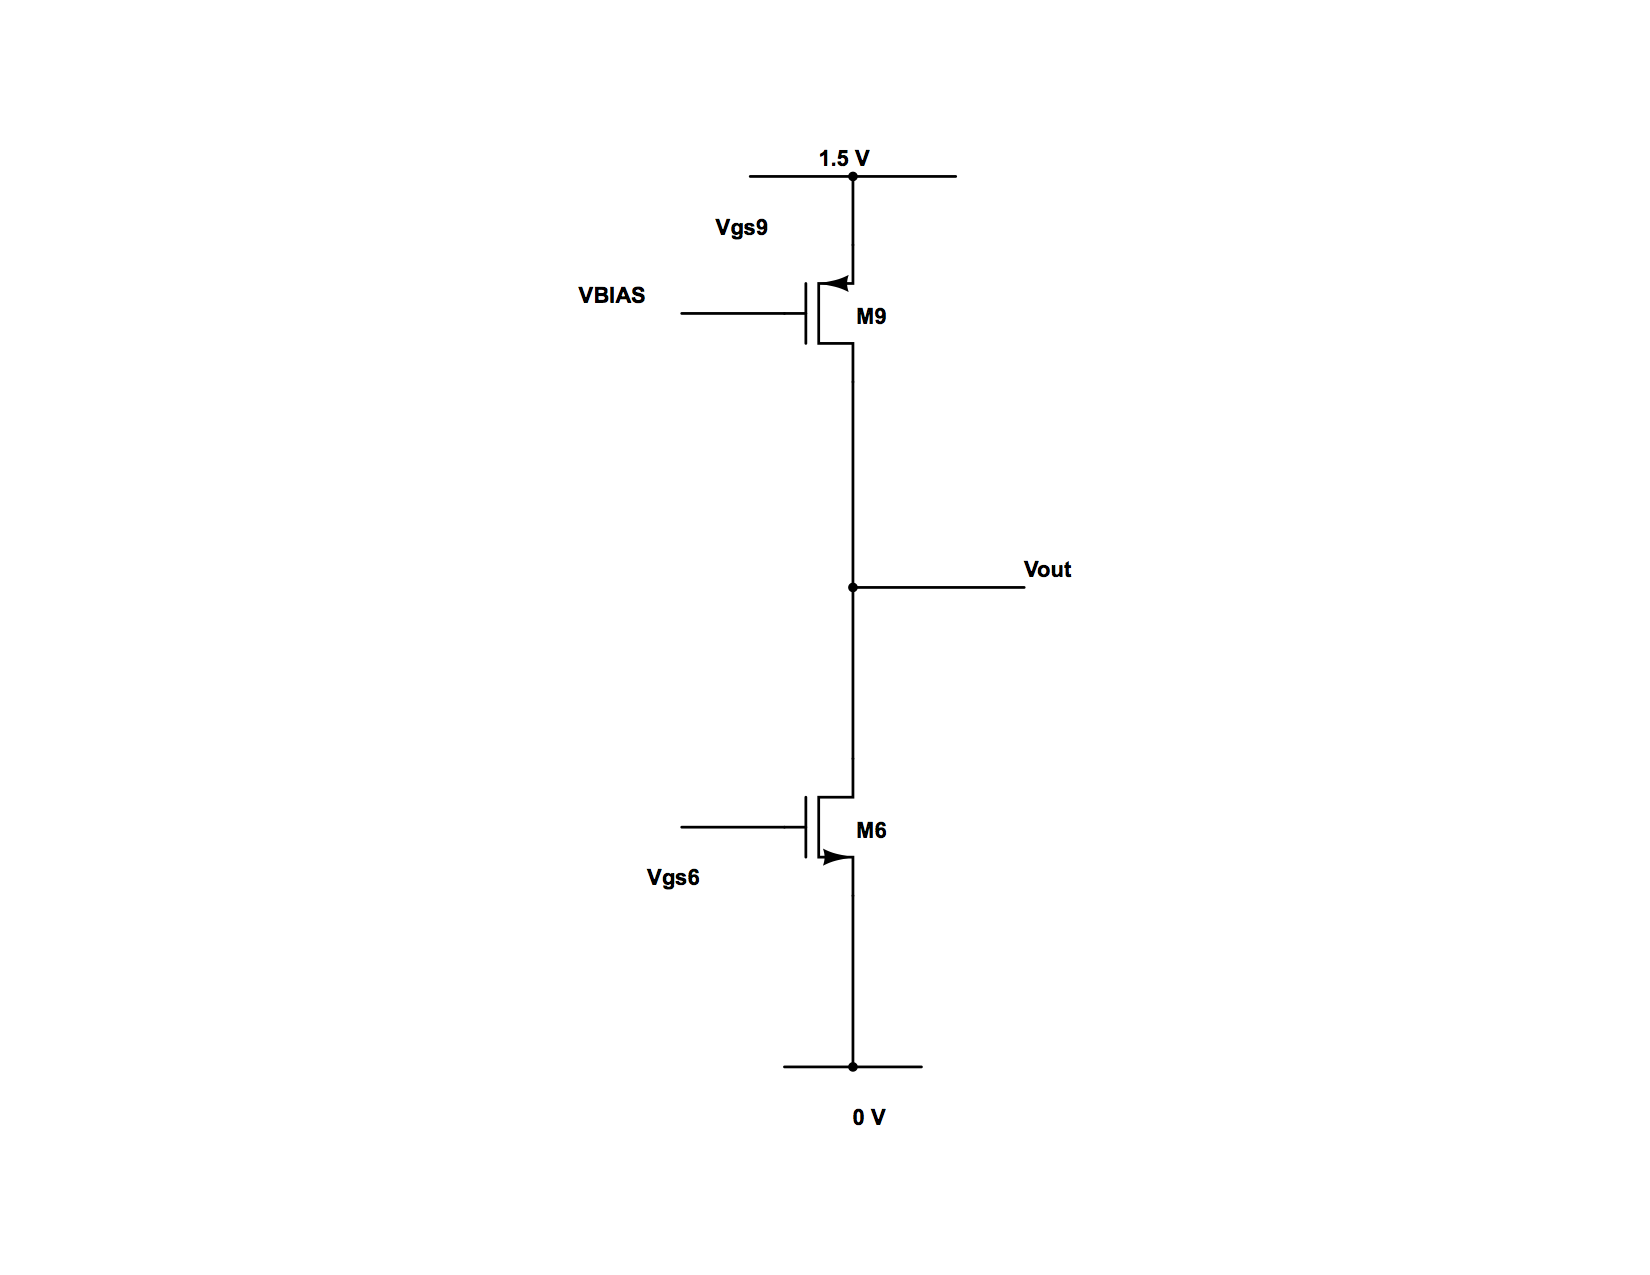
\includegraphics[width=90mm]{cmos-swing-analysis-second-stage.png}
		\end{center}

		{In order to satisfy an output swing within 0.15 V of the rails, we must satisfy the following conditions: }
		\newline
		\newline
		$$ V_{out, _{max}}  = V_{DD} - V_{ov_{9}} = 1.35 V $$
		$$ V_{out, _{min}}  =  V_{ov_{6}} = 0.15 V$$

		Solving for the upper range...
		$$V_{ov_{9}} \le 0.15 V $$
		$$V_{SG_{9}} - V_{t} \le 0.15 V $$
		$$ V_{SG_{9}} \le 0.45V $$
		Using this, we have a range for $V_{BIAS}$.
		$$ 1.05 V\le V_{BIAS}  < 1.2V $$

		Solving for the lower range...
		$$V_{ov_{6}} \le 0.15 V $$
		$$V_{GS_{6}} - V_{t} \le 0.15 V $$
		$$ V_{GS_{6}} \le 0.45V $$
		$$ 0.3 V< V_{G_{6}}  \le 0.45V $$
		\newline
		
		\pagebreak

	\item % 2
		{\bf Common Mode Input Range}
		\newline
		\begin{center}
		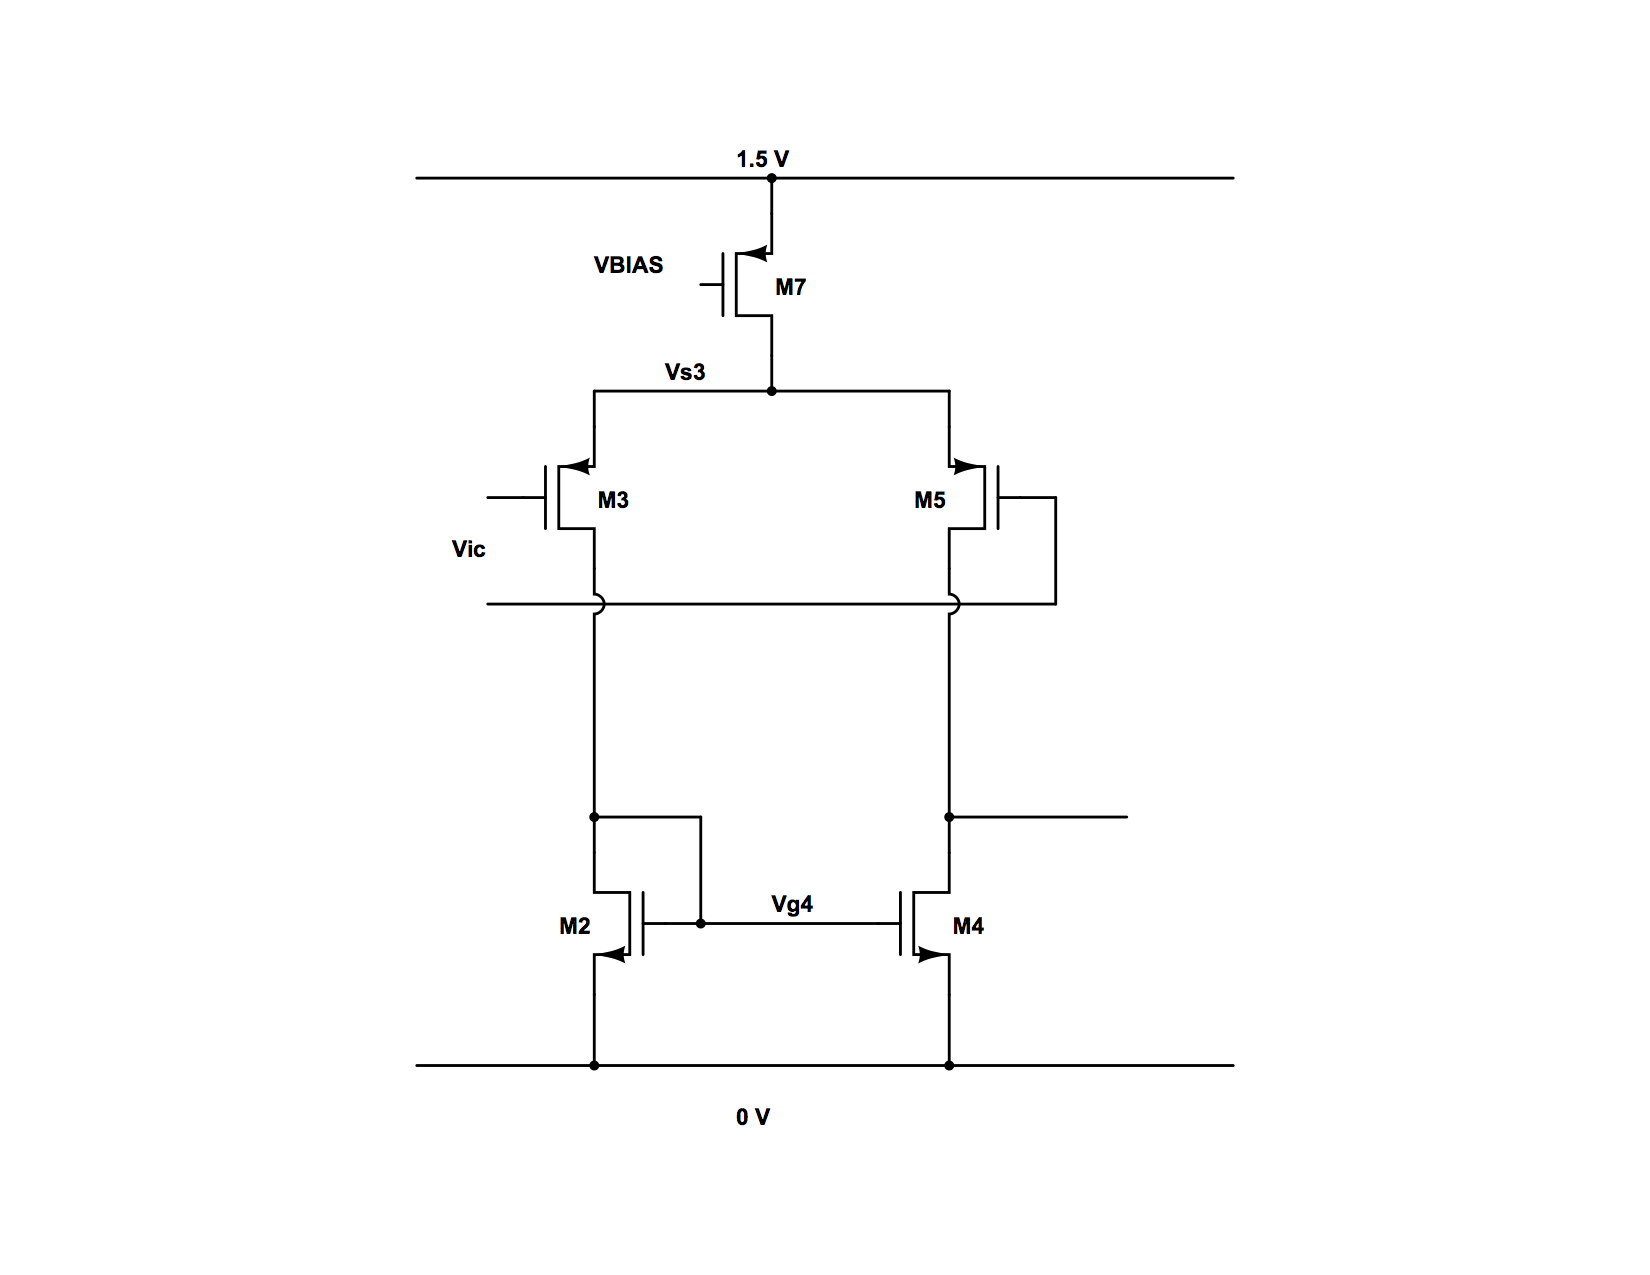
\includegraphics[width = 90mm]{common-mode-input-range-analysis.png}
		\end{center}

		{With pure common mode input, we have the following: }

		$$ V_{DS_{4}} = V_{DS_{2}} = V_{t_{2}}+V_{ov_{2}} $$
		$$ V_{GD_{3}} = V_{GD_{5}} = V_{IC} - V_{t_{2}} -V_{ov_{2}} $$
		When $V_{IC}$ is reduced to the point where $ V_{GD_{3}} = V_{GD_{5}}  = V_{t_{3}} = V_{t_{5}}, M3 $ and $ M5 $ operate at the edge of saturation. 
		Thus, we define the lower end
		of the common mode input range to be :

		$$ V_{IC} \ge V_{t_{3}} + V_{t_{2}}+V_{ov_{2}}  $$
		$$ V_{IC} \ge V_{ov_{2}}  $$

		The specification calls for a common mode input range that is $ 0.8V $ inside the output swing range. This gives us a constraint on $  V_{ov_{2}} $

		$$ V_{IC_{min}} = 0.15 V $$
		$$ V_{ov_{2}}  \le 0.15V$$

		If $ V_{IC} $ is too high, we have $M7$ falling into the triode region. Consider the drain voltage of $ M7: $

		$$ V_{DS_{7}} = V_{IC} - V_{GS_{3}} -V_{DD} = V_{IC} - V_{t3} - V_{ov_{3}} - V_{DD} $$

		Therefore, $ V_{IC} $ must satisfy the following:

		$$ V_{IC} < V_{DD_{}}  -	| V_{t_{3}}| - |V_{ov_{3}}| - |V_{ov_{7}}| $$
		$$ V_{IC} < 1.5  -0.3 - |V_{ov_{3}}| - 0.15 $$
		$$ V_{IC} < 1.05 - |V_{ov_{3}}|  $$
		From the specification,
		$$V_{IC_{max}} = 0.95 V$$
		$$ 0.95 < 1.05 - |V_{ov_{3}}|  $$
		$$ |V_{ov_{3}}| < 0.100 $$

		\pagebreak

	\item % 3

		{\bf Differential Gain}
		\newline
		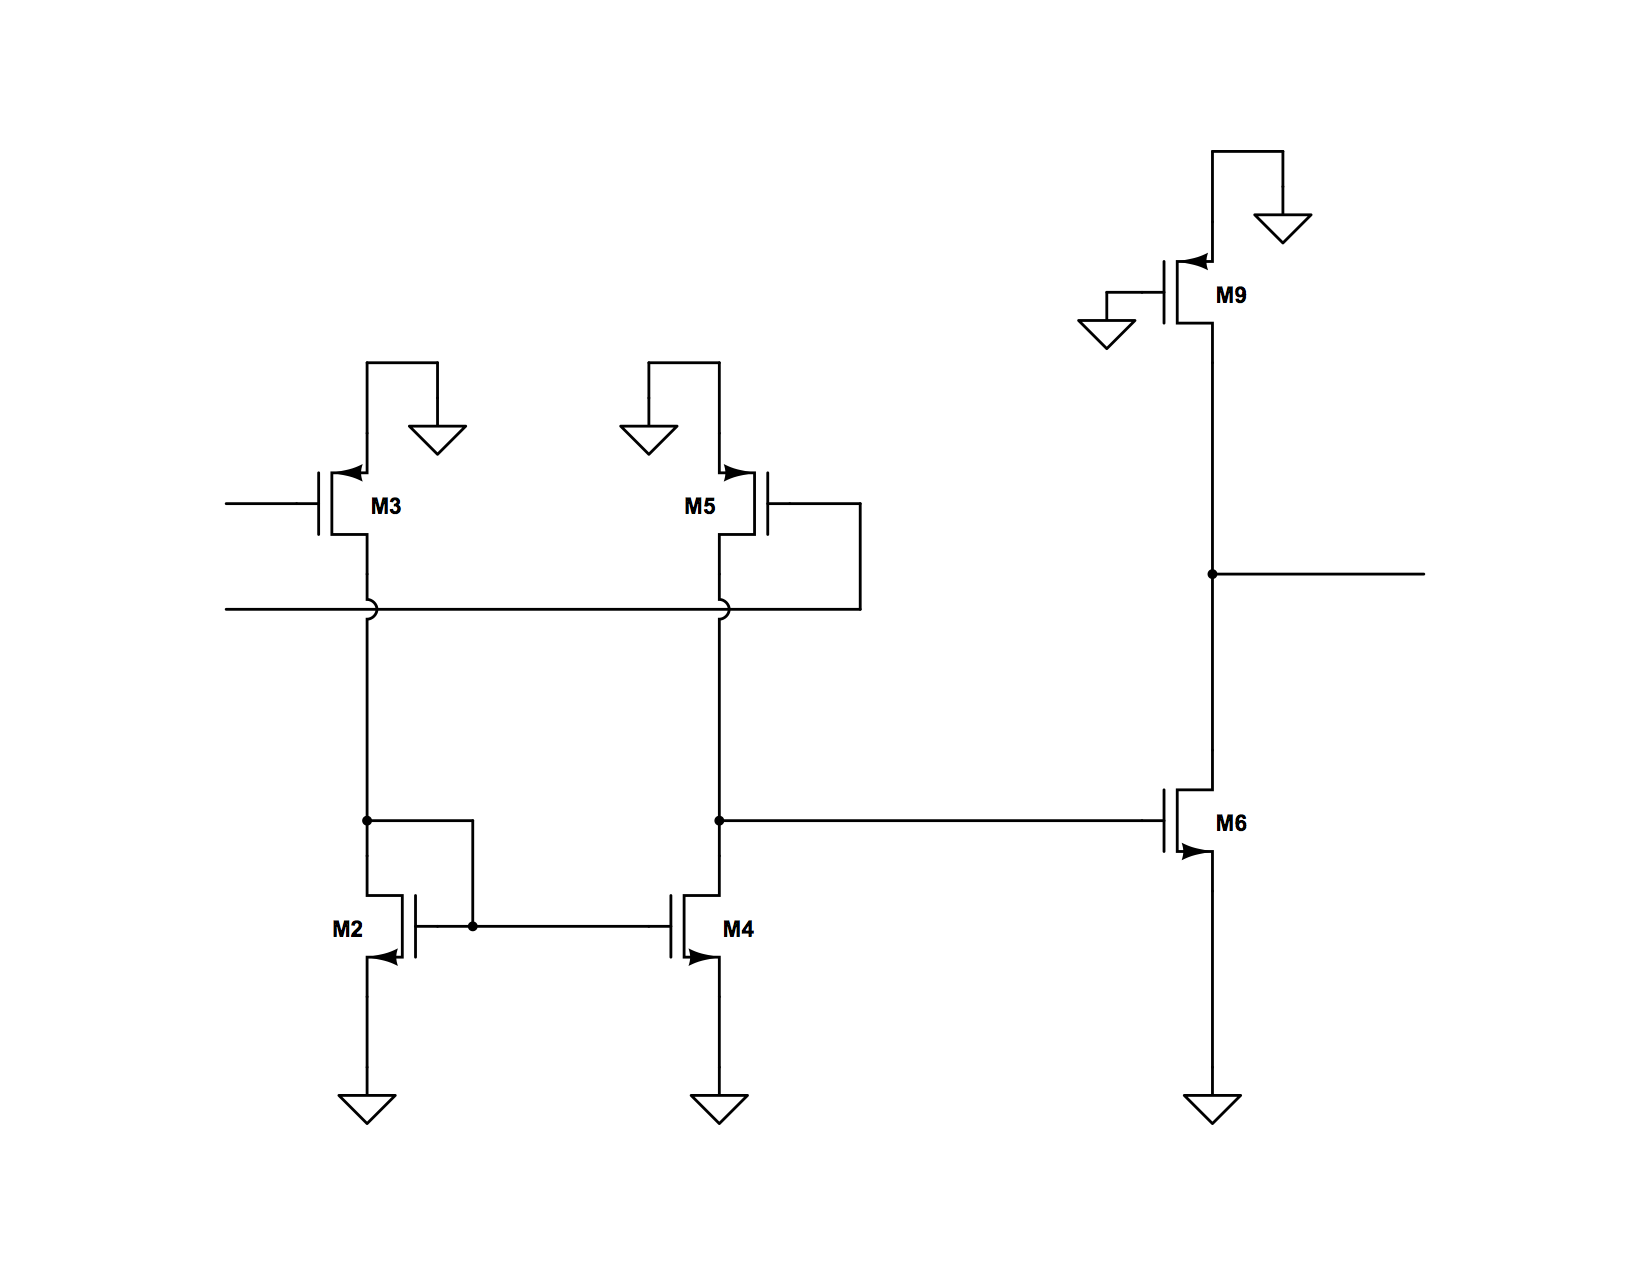
\includegraphics[width=100mm]{cmos-ss-model.png}
		\newline
		\newline
		Total Gain: $A_{v} = A_{v_{1}}A_{v_{2}}$

		$$ A_{v_{1}} = gm_{3}\left(\frac{\frac{V_{A4}}{I_{D3}}\frac{V_{A5}}{I_{D3}}}{\frac{V_{A4}}{I_{D3}}+\frac{V_{A5}}{I_{D3}}}\right) \ \ \ \ \ \ \ \ \ \ A_{v_{2}} = -gm_{6}\left(\frac{\frac{V_{A6}}{I_{D6}}\frac{V_{A9}}{I_{D6}}}{\frac{V_{A6}}{I_{D6}}+\frac{V_{A9}}{I_{D6}}}\right)$$
		\newline
		$$ A_{v} = \frac{-gm_{3}gm_{6}}{I_{D3}I_{D6}}\left(\frac{V_{A4}V_{A5}}{V_{A4}+V_{A5}}\right)\left(\frac{V_{A6}V_{A9}}{V_{A6}+V_{A9}}\right) $$
		\newline
		Using the relation $ \frac{gm}{I_{D}} = \frac{2}{r_{0}} $ gives us
		\newline
		$$ A_{v} = \frac{-4}{V_{ov3}V_{ov6}}\left(\frac{\frac{1}{\lambda_{n}}\frac{1}{\lambda_{p}}}{\frac{1}{\lambda_{n}}+\frac{1}{\lambda_{p}}}\right)^2$$

		A $V_{ov6}$ of 0.15V and a $V_{ov_{3}}$ of 0.1V gives us a differential mode gain of
		$$ A_{v} = -2166 $$ 
		
		\pagebreak

	\item %4

		{\bf CMRR}
		\newline
		\begin{center}
		CMRR = $|\frac{A_{dm}}{A{cm}}|$
		\end{center}
		
		The common mode rejection ratio is only dependent upon the first stage of the amplifier, because the second stage is a single ended input and output.
		\newline
		\begin{center}
			CMRR = $2gm_{3}r_{07}gm_{2}(r_{03} || r_{02})$

			= $\frac{4}{V_{ov3}V_{ov2}}\left(\frac{\frac{1}{\lambda_{n}}\frac{1}{\lambda_{p}}}{\frac{1}{\lambda_{n}}+\frac{1}{\lambda_{p}}}\right)$

		\end{center}
		The specification calls for a CMRR that is $\ge$ 75 dB.

		With $V_{ov3}$ set to 0.1V we get
		$$ 5623.4 = \frac{4*2.857}{0.1*V_{ov2}} $$
		$$ V_{ov2} = 0.0203V $$

		\pagebreak


	\item %5
		{\bf $ \left(\frac{W}{L}\right) $ Ratios}
		\newline

		Here, we set the bias current $I_{BIAS} = 9$ $ \mu A $ and estimate the optimum device dimensions that minimize channel lengths and come within acceptable margins of the expected values.

		Decreasing $V_{ov7}$ to 0.1V and knowing the drain of $M7$ must sustain a voltage of at least 0.55V to satisfy the common mode input range specification gives us the following

		$$ \frac{1}{2}k_{p}'\frac{W}{L}_{7}(V_{ov7})^2(1+\lambda_{p}V_{SD}) = 9\mu A $$
		$$ \frac{1}{2}132.8\times10^{-6}\frac{W}{L}_{7}(0.1)^2(1+0.15(1.5-0.55)) = 9\mu A $$
		$$ \frac{W}{L}_{7} = 11.86$$
		\newline

		With $V_{ov3} = 0.1V $ and the drain of $M3$ constrained to 0.32V gives us
		$$ \frac{1}{2}k_{p}'\frac{W}{L}_{3}(V_{ov3})^2(1+\lambda_{p}V_{SD}) = 4.5\mu A $$
		$$ \frac{1}{2}132.8\times10^{-6}\frac{W}{L}_{3}(0.1)^2(1+0.15(0.55-0.3203)) = 9\mu A $$

		$$ \frac{W}{L}_{3} = 6.55$$
		\newline

		Solving for $M2$, with $V_{ov2} = 0.0203 $ and $V_{DS}$ = 0.0203 + $V_{t}$

		$$ \frac{1}{2}k_{n}'\frac{W}{L}_{2}(V_{ov2})^2(1+\lambda_{p}V_{DS}) = 4.5\mu A $$
		$$ \frac{1}{2}332\times10^{-6}\frac{W}{L}_{2}(0.0203)^2(1+0.2(0.3203)) = 4.5\mu A $$

		$$ \frac{W}{L}_{2} = 61.82$$
		\newline

		With $M9$ the same size as $M1$ we have

		$$ \frac{1}{2}k_{n}'\frac{W}{L}_{6}(V_{ov6})^2(1+\lambda_{n}V_{DS}) = 9\mu A $$
		Here we set the DC voltage at the output to be $\frac{V_{DD}}{2} = 0.75V$
		$$ \frac{1}{2}332\times10^{-6}\frac{W}{L}_{6}(0.387-0.3)^2(1+0.2(0.75)) = 9\mu A $$

		$$ \frac{W}{L}_{6} = 6.23$$

		Device dimensions:
		$$ \frac{W}{L}_{1} = 11.86 \ \ \ \ \ \ \ \ \ \ \ \ \frac{W}{L}_{7} = 11.86$$
		$$ \frac{W}{L}_{3} = 6.55  \ \ \ \ \ \ \ \ \ \ \ \  \frac{W}{L}_{5} = 6.55$$
		$$ \frac{W}{L}_{2} = 61.8 \ \ \ \ \ \ \ \ \ \ \ \  \frac{W}{L}_{4} = 61.8$$
		$$\frac{W}{L}_{6} = 6.23$$
		$$\frac{W}{L}_{9} = 11.86$$


		%$$ \frac{W}{L}_{1} = \frac{5460}{325} \ \ \ \ \ \ \ \ \ \ \ \ \frac{W}{L}_{7} = \frac{5460}{325}$$

		%$$ \frac{W}{L}_{3} = \frac{520}{195}  \ \ \ \ \ \ \ \ \ \ \ \  \frac{W}{L}_{5} = \frac{520}{195}$$

		%$$ \frac{W}{L}_{2} = \frac{715}{130} \ \ \ \ \ \ \ \ \ \ \ \  \frac{W}{L}_{4} = \frac{715}{130}$$

		%$$\frac{W}{L}_{6} = \frac{715}{260}$$

		%$$\frac{W}{L}_{9} = \frac{520}{195}$$

		\pagebreak

	\item %6
		{\bf Power Supply Rejection Ratio}
		\newline

		In calculating the PSRR, we will neglect the variations due to the positive supply, $V_{DD}$. This is because $PSRR_{+}\rightarrow \infty $ for low frequencies with perfect matching. This analysis is shown in G$\&$M page 431.

		Instead, we will calculate the PSRR that emerges due to variations from the $V_{SS}$ supply, which in this case is ground.

		\begin{center} 
			$$A_{-} = \frac{v_{o}}{vss} = \frac{r_{09}}{r_{06}+r_{09}} = \frac{\frac{1}{\lambda_{p}}}{\frac{1}{\lambda_{n}}+\frac{1}{\lambda_{p}}}$$

			$$PSRR = \frac{A_{dm}}{A_{-}} = \frac{2166}{0.5714}$$
			$$ = 3790.5$$
			= 71.5 dB 

			71.5 dB $>$ 60 dB
		\end{center} 
		\pagebreak

	\item %7

		{\bf Power Dissipation}
		\newline

		With $9\mu A$ of current running through each branch, we have a total of $27 \mu A$ running through the entire circuit.
		$$ P = IV$$
		$$ = 27 \mu A \times 1.5V $$
		$$ = 40.5 \mu W $$

		\begin{center}
			40.5$\mu$W $<$1.5 mW
		\end{center}
		
	\pagebreak	

\end{enumerate}


\end{document}